\section{Data}
\label{sec:data}
The data were collected from the public part of the HackerOne website. From 35 public bounty programs, we collected the rewards received by security researchers (in US dollars), with their timestamps (45 other public bounty programs do not disclose detailed information on rewards, and the number of private programs is not disclosed). Since HackerOne started its platform in December 2013, new public programs have been launched roughly every two months, following an essentially memoryless Poisson process ($\lambda = 57$ days, $p < 0.001$ and $R^2 > 0.99$). Figure \ref{timeline}A shows the timeline of the 9 most active programs with at least 90 valid (i.e., rewarded) bug discoveries, as of February 15, 2016. When a new program is launched, we observe an initial peak within weeks after launch, which accounts for the majority of discoveries. Following the initial surge of vulnerability discoveries, bounty awards become less frequent following a decay function with long-memory, following a robust power law decay $\sim t^{\alpha}$ with $\alpha = -0.40(4)$ ($p < 0.001$ and $R^2 = 0.79$) at the aggregate level and over all 35 bounty programs (see Figure \ref{timeline}B). Some programs depart from this averaged trend: For instance Twitter exhibits a steady, almost constant, bug discovery rate and VKontakte exhibits its peak activity months after the initial launch. These peculiar behaviors may be attributed to program tuning and marketing, to sudden change of media exposure or even to fundamental differences of program comparative fitness, for which we do not have specific information.\\

\begin{figure}[h]
\begin{center}
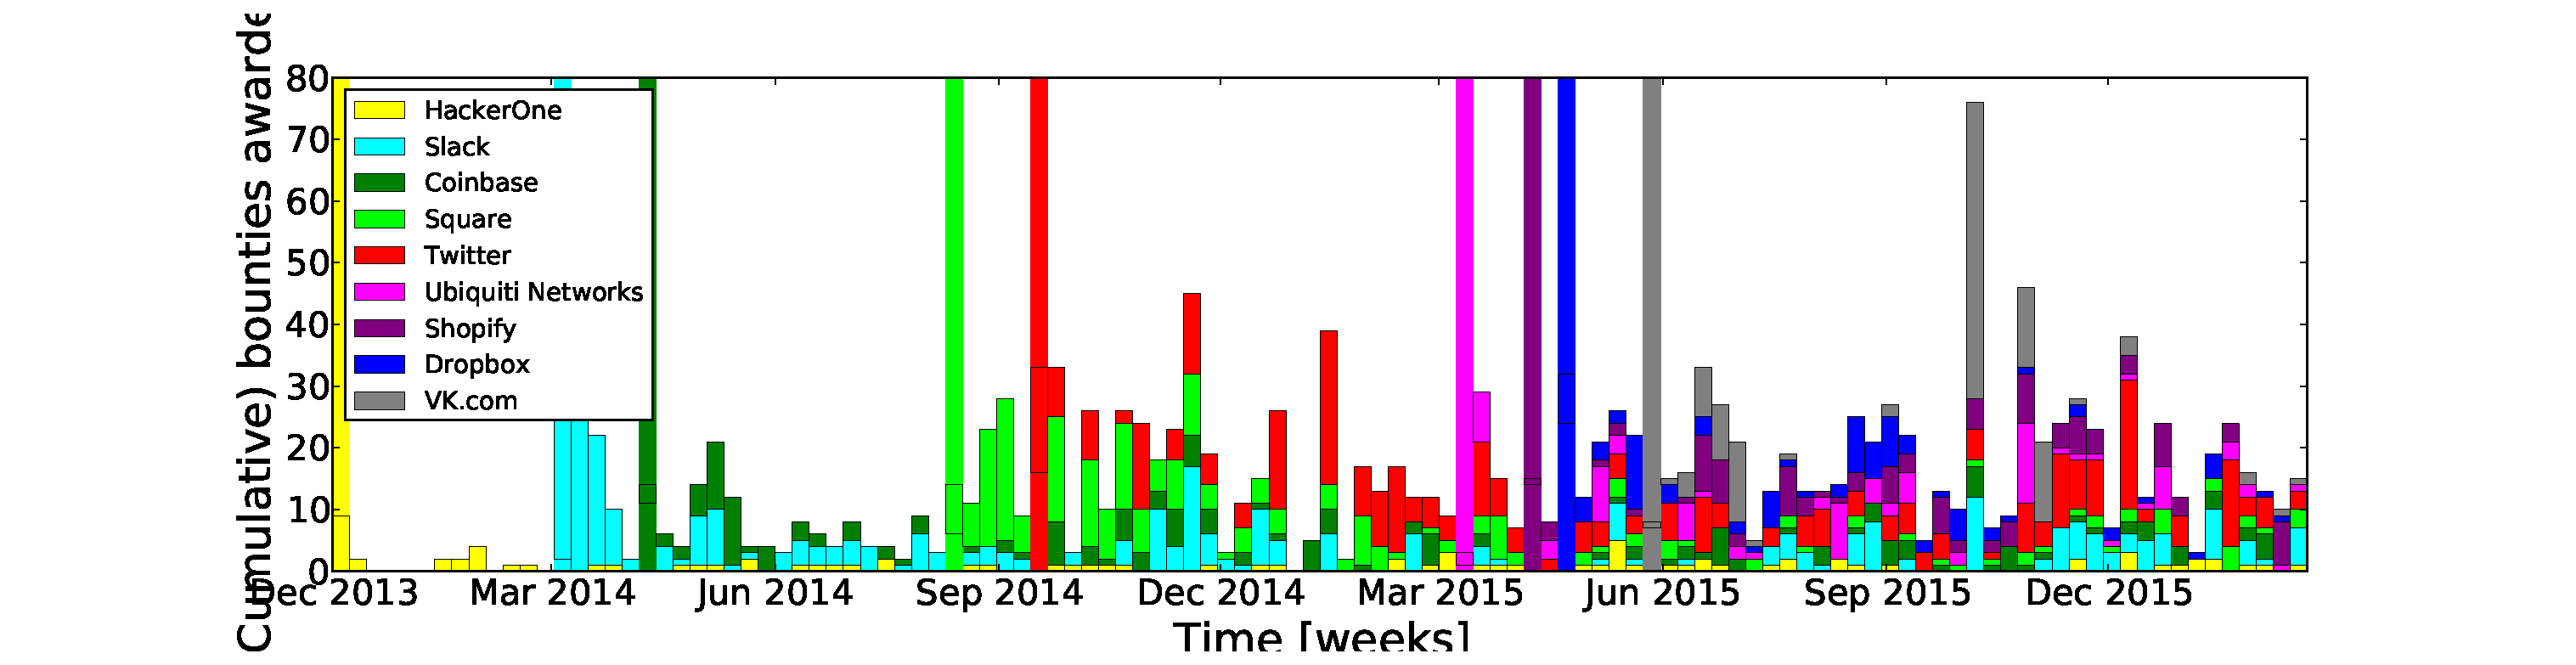
\includegraphics[width=12cm]{../figures/timeline.eps}
\caption{\footnotesize {\bf A.} Weekly vulnerability discoveries for the 9 most active programs (with at least 90 bug discoveries as of February 15, 2016). The light colored vertical bars represent the start of the program, occurring when the first bounty is awarded. Most programs exhibit an initial shock, followed by a decay of discoveries, which is characterized at the aggregate level by a long-memory process (panel {\bf B}) characterized by a power law decay $\sim t^{\alpha}$ with $\alpha = -0.40(4)$ ($p < 0.001$ and $R^2 = 0.79$). Each data point in the figure is the median of normalized vulnerability numbers of all 35 programs considered in this study.}
\label{timeline}
\end{center}
\end{figure}

The long-memory process of bug discovery following the launch of a bug bounty program (c.f., Figure \ref{timeline}B) is compatible with the long-established $\sim 1/\tau$ law of bug discovery in software testing \cite{adams1984textordfeminineoptimizing}. The difference of exponent $\alpha \approx 1$ instead of $1$. in the $\sim 1/\tau$ law of software reliabiltiy, $\tau$ refers to testing time, i.e., the number of tests to perform, in order to reach a given reliability level. The long-memory process associated with the decay of bug discovery (c.f., Figure \ref{timeline}B) is presented in absolute time. Long-memory processes associated with human behaviors are often associated with  human timing effects, which correspond to task priority queueing and a rationalize use of time as non-storable scarce resource \cite{maillart2011quantification}. Long-memory processes observed in human behaviors are also associated with critical cascades of events. {\bf Self-excited Hawkes Process with power law kernel (following human timing)\cite{sornette2014much}. Here, the rationale for cascades builds on 2 ingredients : (i) each security researcher generates a cascade of bug discoveries, and (ii) each bug discovery attracts new security researchers, who in turn trigger their own bug discovery cascade. Cascades are typically slightly heavy-tailed, however bounded, as we'll later : we will dissect these cascades in conjunction with incentives provided by the accumulation of bounties (reputation, slight chance to find less obvious bugs bring more reputation, and increased bounties rewards)}.


\sout{: When the program launches, it takes some time first for the researcher to be exposed to the new program (through the media and social media), second for the researcher to find and submit bugs, and third for the organization managing the bug bounty program to assess the quality of each submission, and assign a proper reward. To account for all these delays, one may resort to priority queueing applied to humans: First, competing attention prevents immediate exposure to the news of a new program; Second, when security researchers get interested in a new program, they may still be actively searching bugs on other programs or performing other tasks (such as e.g., their regular job, leisure, family matters); Third, when subjected to a flow of bug submissions, security teams at organizations leading bug bounty programs assign priorities among submissions, and resolve them with human resources available at the time of submission. }

\sout{These delays are best rationalized by human timing contingencies, and moreover, by an economy of time as a scarce, non-storable resource, which is known to generate long-memory responses of the form $\sim t^{-1.5}$ between the arrival and the execution of a task \cite{maillart2011quantification}. The observed much slower decay may result from the compound effect of multiple delays, such as those mentioned above. The initial burst of discoveries, followed by a long-memory decay may also result from the increasing difficulty associated with finding new bugs for each bounty program, as the most obvious vulnerabilities get uncovered first.  Since we consider only the {\it time of discovery} as the moment when the validity of the bug submitted is acknowledged by the program manager, we are mostly blind to the human timing effects associated with the long-memory process observed on Figure \ref{timeline}B, including when submissions are made, but don't lead to a discovery associated with a monetary reward.}\\

Here, we don't consider the timing effects encompassing delays, effort, processing time, but rather the incremental valid bug discovery and reporting by security researchers [refine here].

